\documentclass[a4paper,12pt]{article}

% don't forget the document class, generally : \documentclass[a4paper,12pt]{article}

\usepackage[utf8]{inputenc}
\usepackage[french]{babel}
\usepackage{graphicx}
\usepackage{gensymb}
\usepackage{amsmath}
\usepackage{float}
\usepackage{scrextend}
\usepackage{caption} 
\usepackage{siunitx}
\usepackage{enumitem}
\usepackage{amsthm}
\usepackage{fancyhdr}
\usepackage{amssymb}
\usepackage{wrapfig}
\usepackage{geometry}
\usepackage{standalone}
\usepackage{import}
\usepackage[usenames, dvipsnames]{color}

 \usepackage{biblatex} % manages bibliography and references
\addbibresource{sample.bib}


\geometry{hmargin=1in, vmargin=1in}

 \newenvironment{absolutelynopagebreak}
 {\par\nobreak\vfil\penalty0\vfilneg
 \vtop\bgroup}
 {\par\xdef\tpd{\the\prevdepth}\egroup
 \prevdepth=\tpd}
 
 \pagestyle{fancy}                        
\fancyhf{}                               
\fancyhf[HL]{Application des maths}                
\fancyhf[HR]{Géométrie euclidienne}             
\fancyhf[FC]{\thepage/\pageref{Lastpage}}
 
\newtheorem{definition}{Définition}[section]
\newtheorem{theorem}{Théorème}
\newtheorem{corollary}{Corollaire}[theorem]
\newtheorem{lemma}[theorem]{Lemme}
\newtheorem*{hyp}{Hypothèse}
\newtheorem*{concl}{Conclusion}
\newtheorem*{remark}{Remarque}

\captionsetup{format=default,labelformat=simple,labelsep=colon,
justification=justified,font={sf,small},labelfont=bf,
textfont=default} 



\begin{document}
\pagebreak
\subsection{Théorème des médiatrices}

\begin{theorem}
La médiatrice d'un segment est le lieu géométrique des points équidistants à ses extrémités.
\end{theorem}

%insert figure

Pour démontrer ce théorème, nous devons prouver les deux affirmations suivantes:
\begin{enumerate}
    \item Tout point se situant sur la médiatrice d'un segment se situe à la même distance de ses deux extrémités.
    \item Tout point se trouvant à égale distance de deux autres points se situe sur la médiatrice du segment défini par ces derniers.\\
\end{enumerate}


\begin{enumerate}
    \item \begin{proof}
    Nous considérons le segment $AB$, ayant $m$ comme médiatrice. $M$ est le point à l'intersection de $m$ et du segment $AB$.
    
    \begin{hyp}
    $P \in m$ 
    \end{hyp}
    \begin{concl}
    $AP \equiv BP$
    \end{concl}
     
    Grâce au premier cas d'isométrie des triangles, nous observons que les triangles $\triangle AMP$ et $\triangle BMP$ sont isométriques car ils ont un côté en commun ($MP$) et que $AM$ et $MB$ sont isométriques. Par conséquent, $AP \equiv BP$.
     \end{proof}
     
      \begin{figure}[H]
        \centering
        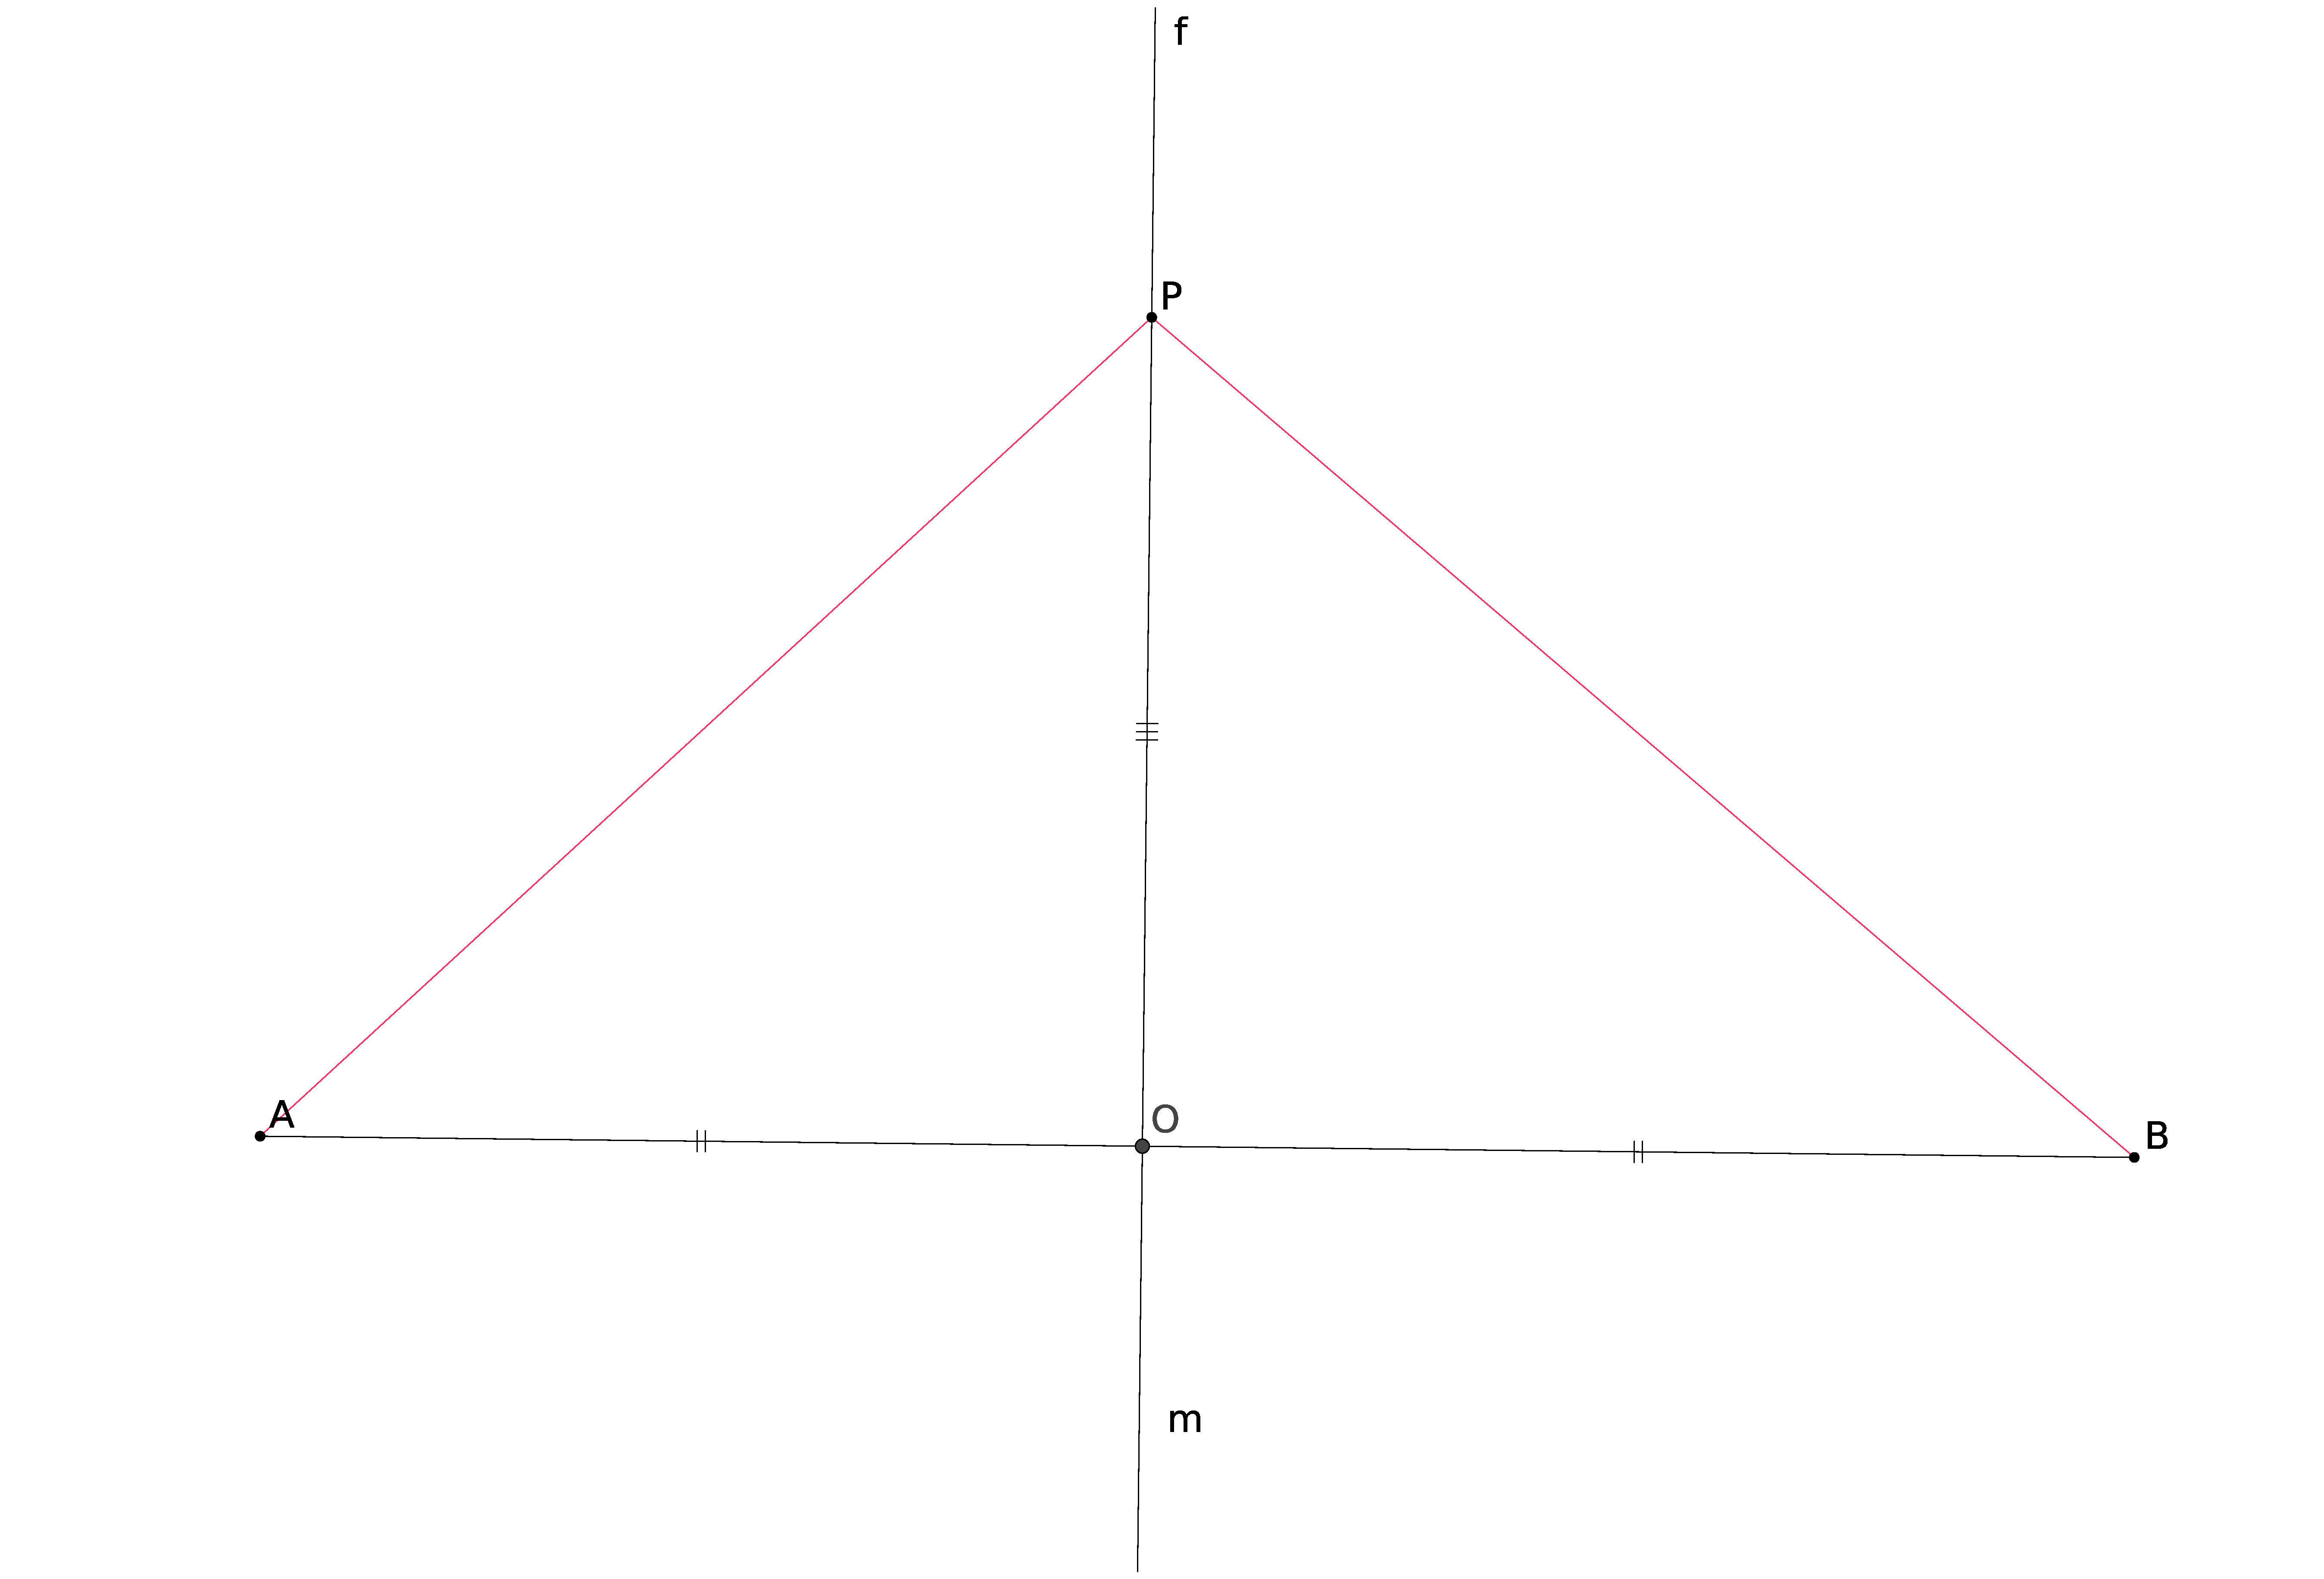
\includegraphics[scale=0.17]{mediatrice1.eps}
    \end{figure}
    
    
     
    \item \begin{proof}
         Nous considérons un point $P$ à égale distance de deux autres point, $A$ et $B$. 
        
        \begin{hyp}
        $AP \equiv BP$
        \end{hyp}
        \begin{concl}
        $P \in m$
        \end{concl}
        Nous traçons le segment $MP$ et observons que c'est la médiane du triangle formé par les points $A$, $P$ et $B$, car il part        de l'un des sommet du triangle et partage le côté opposé en deux parties égales. 
        
       
        
        \begin{figure}[H]
        \centering
        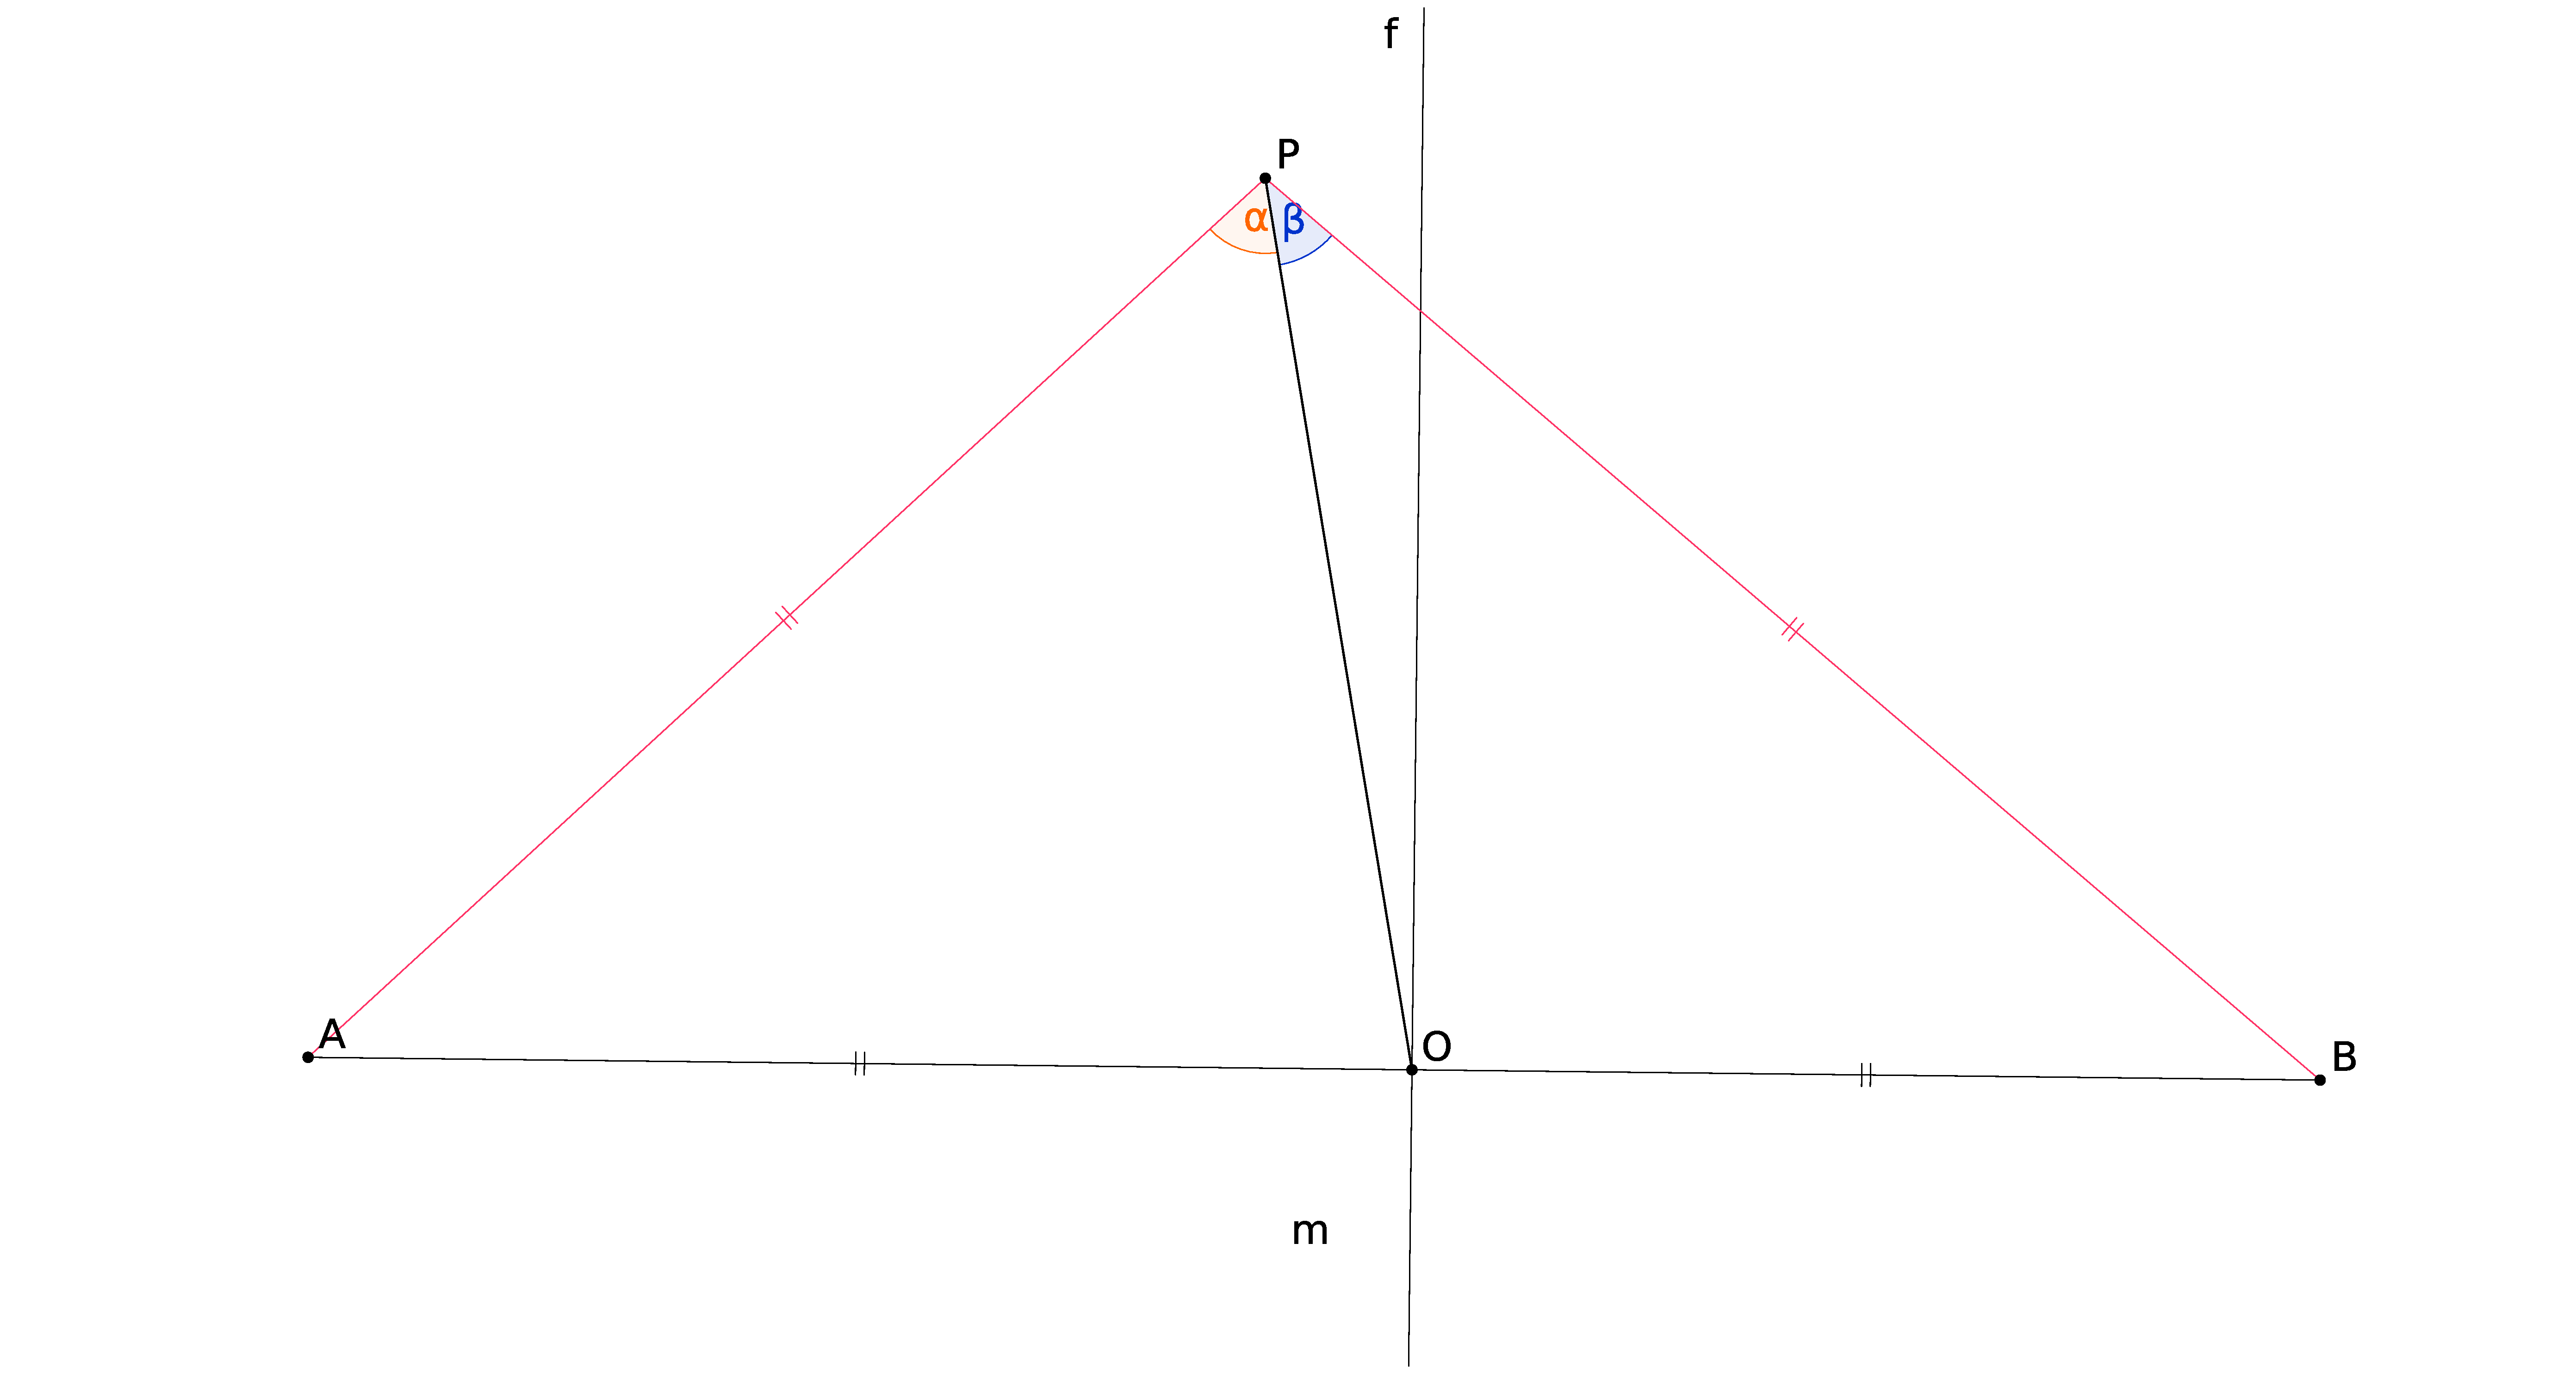
\includegraphics[scale=0.17]{mediatrice2.eps}
    \end{figure}
        
        Ainsi, nous observons que les angles $\angle      APM$ et $\angle MPB$ sont isométriques.  Par conséquent, les triangles $\triangle AMP$ et $\triangle BMP$ sont isométriques      car ils possèdent un angle isométrique ($\angle APM \equiv \angle MPB$) compris entre deux côtés isométriques ($AP \equiv      BP$, par hypothèse et $MP$ en commun). Finalement, le segment $MP$ et la médiatrice de $AB$ sont confondus et $P \in m$.\\
        \end{proof}
\end{enumerate}

\end{document}